% !TEX root = ./tileheat.tex
\section{Background}
\label{sec:tile:caching}

A \emph{tile cache} is a widely used method for dealing with the bad performance of services that render results from base data on-the-fly, such as WMS and similar services. In the following, we discuss the main concepts (Sections~\ref{sec:tile:pyramid} to~\ref{sec:heatmap:model}) and existing methods (Section~\ref{sec:existing:methods}) in tile caching.

\subsection{The Tile Pyramid}
\label{sec:tile:pyramid}

Tile caches are based on a model called a \emph{tile pyramid}, which subdivides a geographical region into a finite number of subregions using a set of $l$ grids~\cite{decola93}. In Figure~\ref{fig:tilepyramid}, a tile pyramid with three levels is shown. The cells of the grids are called \emph{tiles}, and tiles are indexed by a triple $(i,j,z)$. In this triple $z$ identifies a grid, while $i$ and $j$ represent the row and column in the grid where the tile is located. Each grid is associated with a data set at a particular resolution in meters per pixel. Tiles thus correspond to data at a given resolution, and within a bounding box.

\begin{figure}
\centering
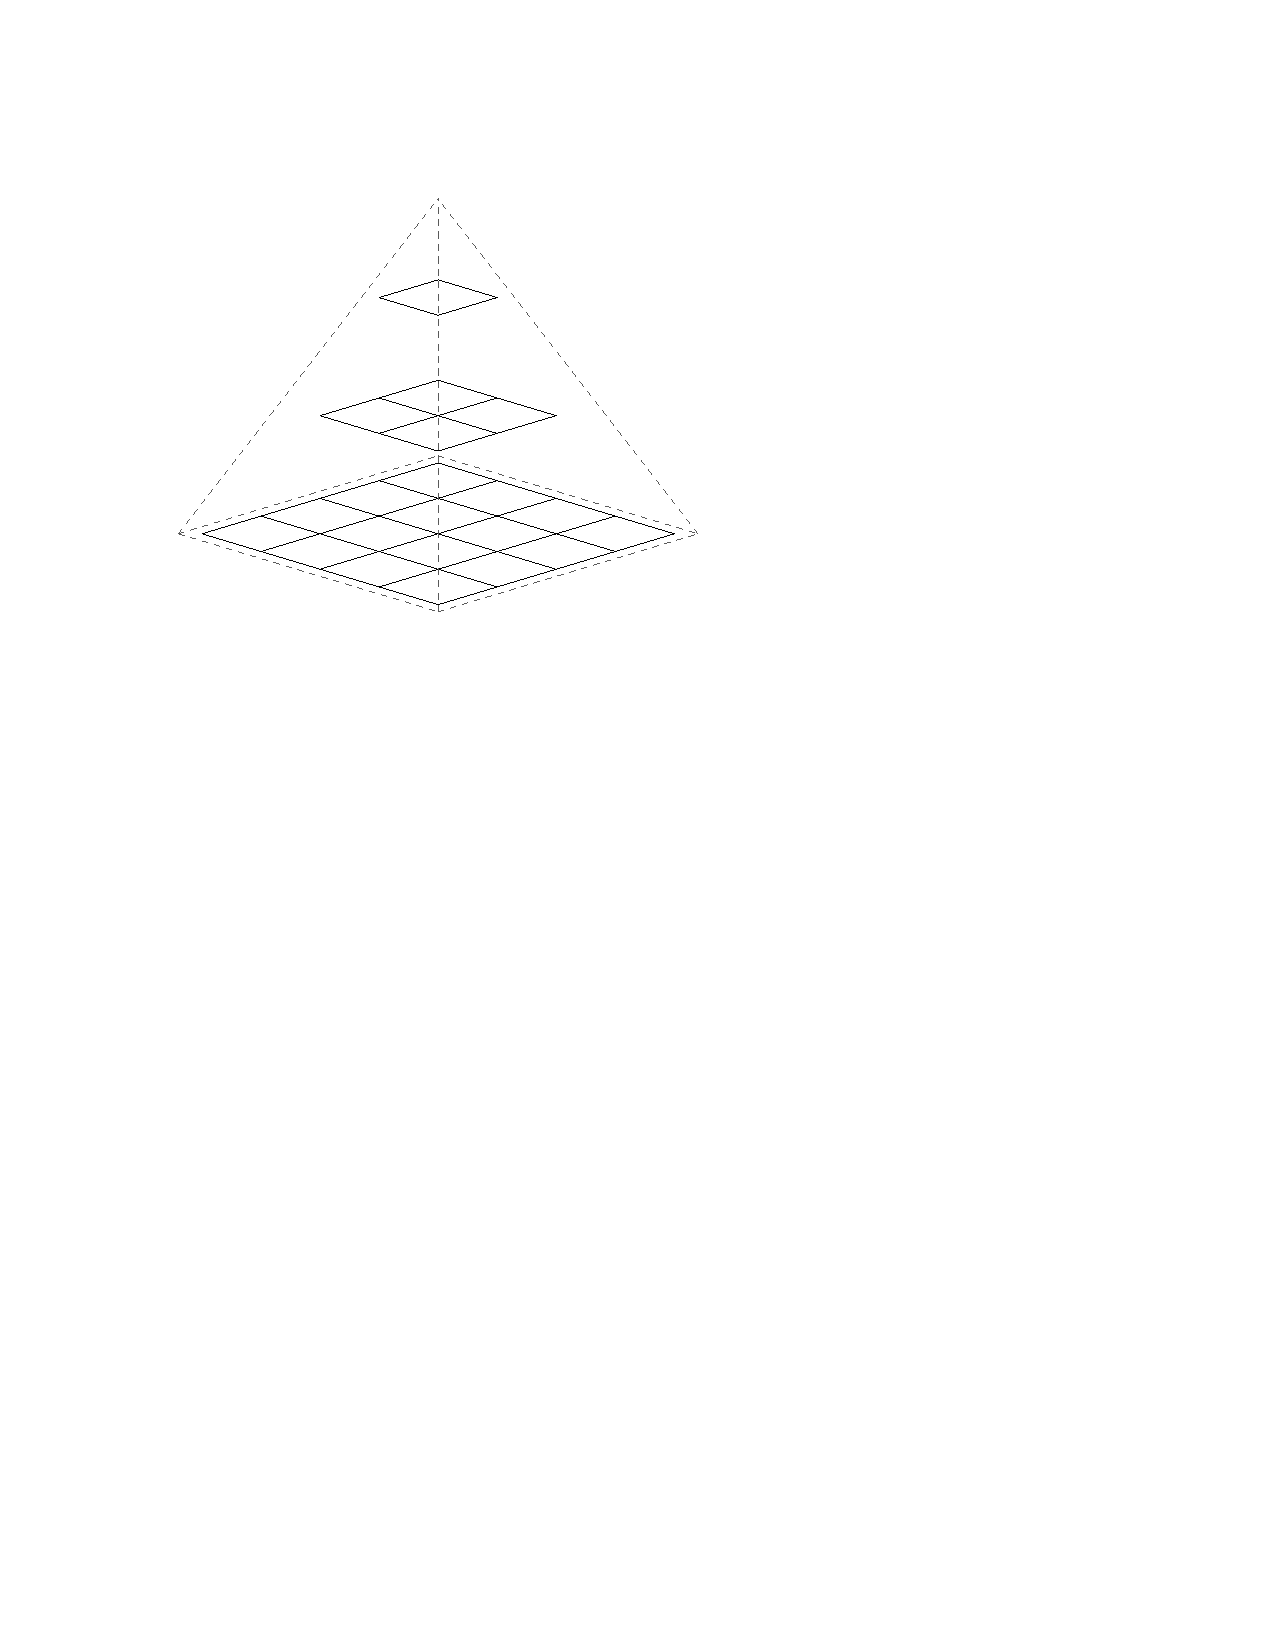
\includegraphics[scale=0.8]{tilepyramid}
\caption{Tile pyramid with three levels $z=\{1, 2, 3\}$ shown. Level $z=1$ has dimensions $(1,1)$. Figure is reproduced from \cite{quinn10}}
\label{fig:tilepyramid}
\end{figure}

When a tile cache is initialized, all tiles point to $null$. A tile is materialized by making it point to geographical data stored on disk. The geographical data is rendered from a set of base objects, and if the base objects are updated the tile becomes \emph{stale}. Stale tiles are removed to avoid serving stale data to clients.

One shortcoming of tile caches is that the number of tiles is exponential in $l$, with grid $i+1$ containing four times as many tiles as grid $i$. This means that a tile cache consumes $O(4^l)$ in storage, and $O(4^l)$ time is required to materialize all tiles. A pyramid of $l=20$ levels requires several petabytes of storage \cite{garcia11}. The throughput of computing tiles has been reported by KMS to be around $58$ tiles per second on their infrastructure \cite{lindegaard12}. At this rate of computing tiles, it would take approximately $200$ years to compute the $3.7 \times 10^{11}$ tiles needed~\cite{garcia11}.

\subsection{Processing user requests}
\label{sec:processing:user:requests}
We abstract user requests to a geospatial web service by two functions: \texttt{GET} and \texttt{PUT}. \texttt{GET} retrieves a tile from a web service, while \texttt{PUT} updates the base data from which tiles are computed. Pseudocode for processing \texttt{GET} and \texttt{PUT} requests are given in Figure \ref{fig:pseudocode}.

\begin{figure}[h]
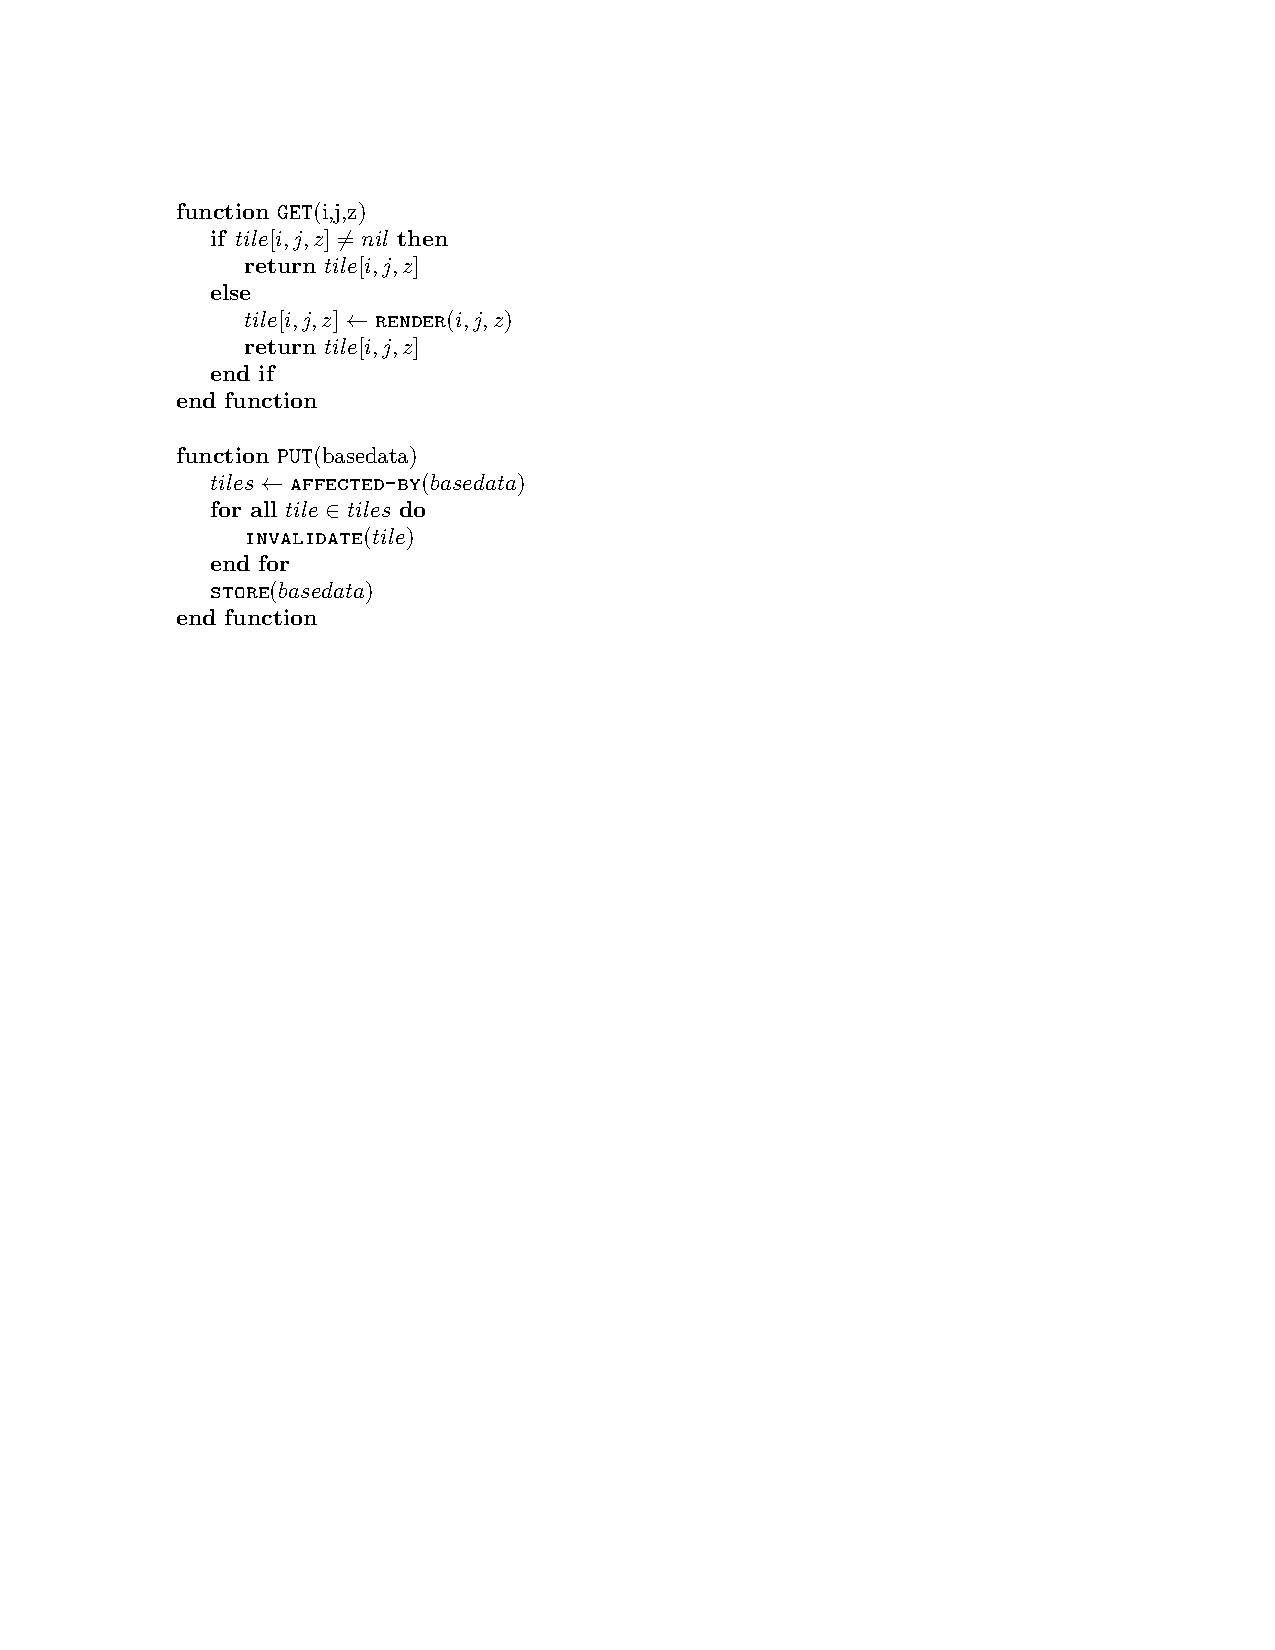
\includegraphics[scale=0.9]{pseudocode}
\caption{Processing a \texttt{GET} request: If the tile is materialized, it is returned. Otherwise it is rendered, stored and returned. Processing a \texttt{PUT} request: When base data is updated, the set of tiles that is affected by the change needs to be invalidated.}
\label{fig:pseudocode}
\end{figure}

An invariant maintained by the above functions is that stale tiles are never returned to the user. However, one implementation difficulty typically encountered in practice is that the method for determining the set of tiles that are affected by an update to the base data is not entirely accurate, i.e., a conservative estimate is used in function \texttt{AFFECTED-BY}. This means that sometimes tiles are unnecessarily discarded.

A bounding box request, such as a WMS request, can easily be modeled as a set of \texttt{GET} requests by computing the set of tiles that are intersected inside the \emph{nearest} grid of the tile pyramid. By nearest, we mean the grid that contains tiles with a resolution that best matches the resolution of the bounding box request. Note that these multiple \texttt{GET} requests must be processed against a consistent snapshot. 
%Description of the appropriate implementation details are however beyond the scope of this paper. 

\subsection{The Heatmap model}
\label{sec:heatmap:model}
Given a set of \texttt{GET} requests, we can generate a heatmap of the requests \cite{fisher07}. A heatmap quantifies the number of requests $h_{i,j,z}^t$ that a tile with index $(i,j,z)$ has received in time period $t$. We consider multi-scale heatmaps, which are associated with a tile pyramid. In this work, we only use heatmaps to measure the number of \texttt{GET} requests per tile, but other request types could also be tracked with heatmaps. For example, we could generate heatmaps of \texttt{INVALIDATE} requests, but this is outside the scope of our work.

\subsection{Existing Methods}
\label{sec:existing:methods}
This section covers existing methods for computing and storing a set of tiles for a tile cache.

\minisec{Parallel processing}
Clearly, we need techniques to speed the computation of a tile cache up, given that the number of tiles in a tile pyramid is huge. Using a parallel programming model such as MapReduce \cite{dean04} could reduce computation time of a tile cache by a large factor, but it would require a significant number of machines. In other words, parallelism improves time-to-solution, but does not reduce the amount of resources necessary for the computation. For organizations such as KMS, this high resource cost renders the use of brute-force parallelism unfeasible. A solution is called for to reduce the number of tiles that needs to be computed --- which could then be orthogonally combined with parallelism if available.

\minisec{Detecting duplicates}
A method that reduces storage requirements is to exploit that many tiles are identical, e.g., blue ocean tiles~\cite{mbtile12}. Unfortunately, this solution does not necessarily reduce computation time, given that tiles often must be computed in order to check that they are duplicates. Heuristics have been suggested to predict these duplicated tiles without full computation, but it is unfortunately not easy to decide with absolute certainty~\cite{mbtile12}. We do not know of any published methods that accurately and efficiently predict whether two tiles are the same in the general case without actually computing them, because arbitrary rendering functions are employed.

\minisec{Tile Caching based on Geometries}
A number of authors have suggested methods for predicting the popularity of tiles. Quinn and Gahegan~\cite{quinn10} suggest using certain classes of base objects, like roads and coastlines, as predictors of where people will look at a map. Tiles that are at most 3 miles away from the selected predictors are cached. Conceptually, this approach is based on a model of rational user behavior with fixed rules, and historical workloads are used only to validate the model.

\minisec{GEOM}
KMS currently uses a simplified version of the approach above, which we term \emph{GEOM}. A set of polygons that roughly cover the land areas of Denmark are used to identify the areas that should be fully materialized at all levels of the tile pyramid (levels 1 to 12). Areas outside of these polygons are only materialized at the top-most levels of the tile pyramid (levels 1 to 6)~\cite{lindegaard12}. The resulting partial cache is manageable in size, as roughly $10\%$ of the tile pyramid is materialized. However, the computation time is reported to be between $1.5$ and $2$ days. Tiles are generated by going row-by-row down the levels of the tile pyramid. This is significantly better than random selection, as the highly popular tiles near the top of the pyramid are generated early.

\section{Analysis}
\label{sec:analysis}

In this section, we analyze the request log of a production geospatial web service within KMS, and observe a number of interesting patterns.
The service we examine is the most popular web service of the The Digital Map Supply, a WMS that receives around 800,000 requests per day, and delivers a general purpose background map of Denmark. We report on both temporal (Section~\ref{sec:temporal:characteristics}) and spatial (Section~\ref{sec:spatial:characteristics}) characteristics of the workload.

\subsection{Temporal characteristics of workload}
\label{sec:temporal:characteristics}

\begin{figure}
\centering
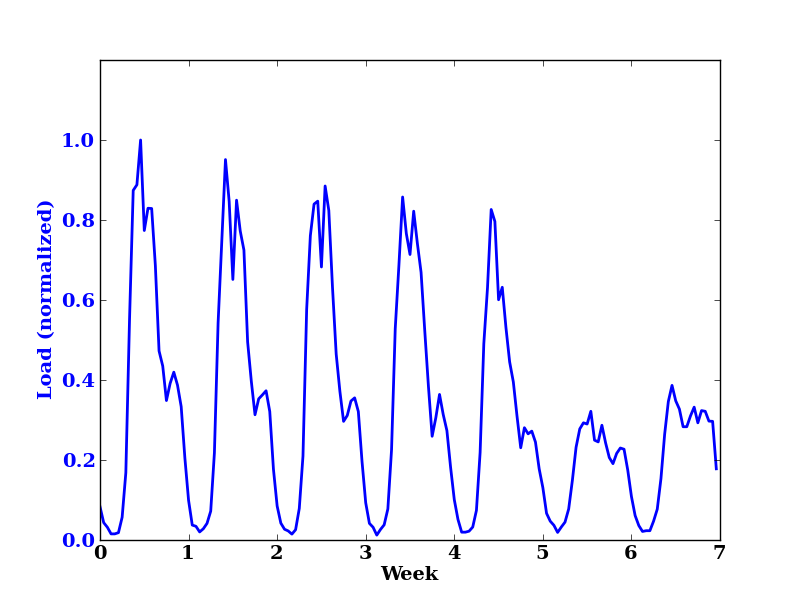
\includegraphics[scale=0.4]{average_load_week.png}
\caption{Average load per hour for each day of the week.}
\label{fig:weekload}
\end{figure}

Using a random sample of 90,000 WMS requests from the log, we analyze the workload over time. We have found the following when examining requests processed per second:

\begin{itemize}
\item The load is consistently higher during the middle part of the day, than during other parts of the day.
\item The 24-hour load curves for any two weekdays are very similar.
\item The 24-hour load curves for Saturdays and Sundays are very similar.
\item In general, the load is much higher during weekdays, compared to weekends.
\end{itemize}

These patterns are shown in Figure~\ref{fig:weekload}, where we display the average 24-hour load curve for each day of the week. The curve is generated as an average of all weeks in the log.

\begin{figure}
\centering
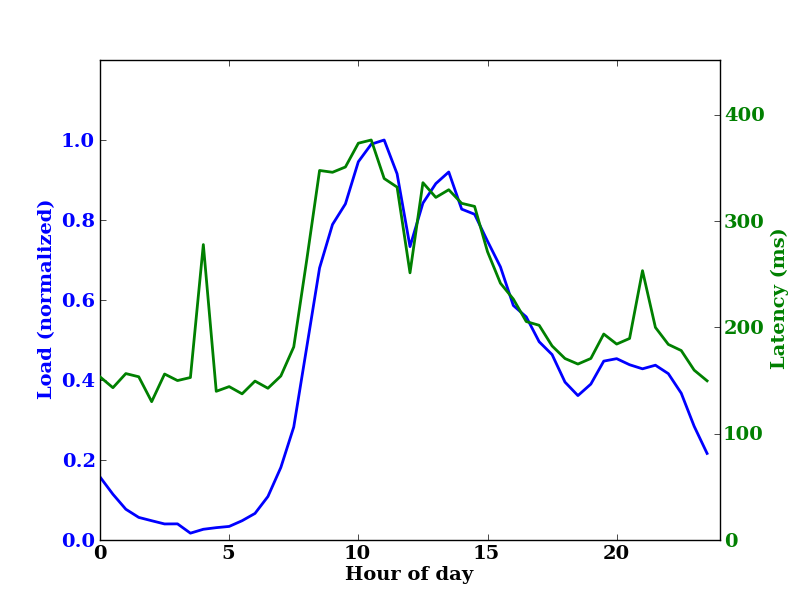
\includegraphics[scale=0.4]{correlation.png}
\caption{The correlation between average load (blue) and average latency (green) for 24-hour period.}
\label{fig:correlation}
\end{figure}

We have also looked at the effect of load on latency. In Figure~\ref{fig:correlation}, we plot, side-by-side, the average load and latency curves for a 24-hour period. We observe the following:

\begin{itemize}
\item Load and latency are highly correlated, especially during the periods of high load.
\item The latency effectively doubles when the load is high.
\item Given that weekdays have higher load than weekends, the degradation of latency is most severe in the middle of the day, on weekdays.
\end{itemize}

Our hypothesis is that the increase in latency is caused by increased concurrency and queueing in the system. We have also tested the stability of the load pattern over time by plotting the load for each day over a longer period within the last quarter of 2011. The load patterns can be seen in Figure~\ref{fig:anomaly}. We observe that in general the load curve is very consistent from one weekday to the next, and one week to the next, but anomalies do occur. During week 49 of the last quarter of 2011, the number of requests suddenly doubles. While it is not easy to know what caused such a load spike, it is interesting to ask whether the spike affects the spatial distribution of requests. We examine this question in Section~\ref{sec:spatial:characteristics}.

\begin{figure}
\centering
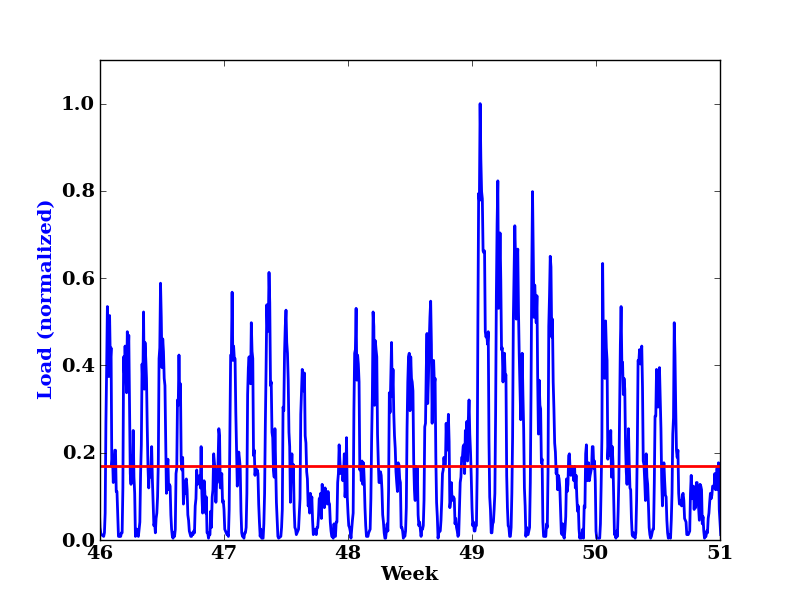
\includegraphics[scale=0.4]{anomaly.png}
\caption{Generally stable load, with an anomaly in week 49. The load almost doubles on the first day of week 49. The red line is the average load.}
\label{fig:anomaly}
\end{figure}

\subsection{Spatial characteristics of workload}
\label{sec:spatial:characteristics}
Using heatmaps we have investigated the spatial distribution of requests. We have selected a large number of weekdays, and extracted a full log for these days. The number of log records is significant, with more than 800,000 requests received per day. In Figure \ref{fig:heatmaps}, we show heatmaps for four of these days. We observe that the spatial distribution of requests is quite similar across days. We observe a similar pattern on other days from the log that we have examined.

Given the anomaly in requests per second that we noted in Figure~\ref{fig:anomaly}, we wanted to investigate if the spatial distribution of requests was different for days of increased load compared to normal days. The lower right part of Figure~\ref{fig:heatmaps} shows a heatmap for the day with unusually high load. The spatial distribution is slightly different compared to the other three heatmaps, but still very similar. The data indicates that the spatial distribution of requests is similar for weekdays, and largely independent of fluctuations in load. Using the notation we defined for heatmaps this means that

\[
h_{i,j,z}^t \approx h_{i,j,z}^{t+1}
\]

\begin{figure}
\centering
\begin{tabular}{|c|c|}
\hline
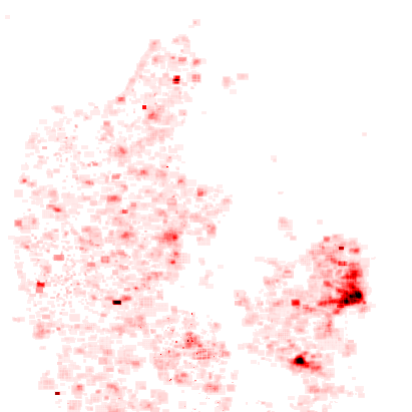
\includegraphics[scale=0.22]{heatmap-e_1.png} & 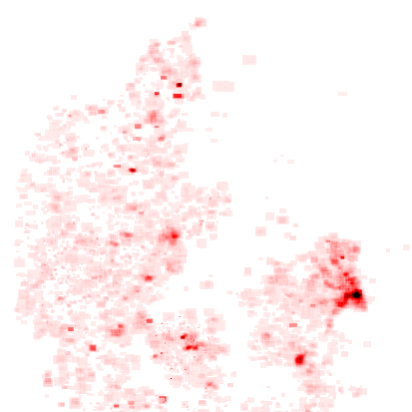
\includegraphics[scale=0.22]{heatmap-e_2.png} \\
\hline
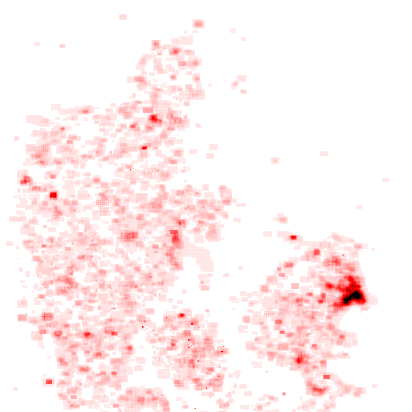
\includegraphics[scale=0.22]{heatmap-e_3.png} & 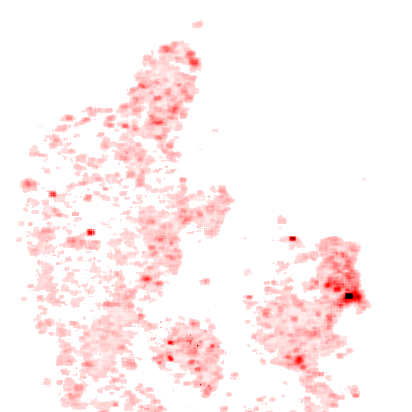
\includegraphics[scale=0.22]{heatmap-e_4.png} \\
\hline
\end{tabular}
\caption{Heatmap of spatial distribution of requests for four consecutive days (resolution $\mathbf{3.2}$ meter/pixel). The spatial distribution is similar but not equal. The day in the lower right corner is the day with very high load identified in Figure \ref{fig:anomaly}.}
\label{fig:heatmaps}
\end{figure}

%In Figure~\ref{fig:skew}, we show the cumulative distribution function of tile access frequencies, which has been computed from the heatmaps. 
We observe that the frequency of tile access is highly skewed; other studies have concluded the same, namely that the spatial distribution of \texttt{GET} requests follows a power law \cite{fisher07,talagala00}. We also observe that the skew increases with resolution, i.e., with  levels of the tile pyramid that contain more tiles. 

In general, this means that the set of tiles needed for a tile cache with a high hit ratio is smaller than one might expect. The main goal of our work and the algorithms we have developed is to explore how small such a cache can be, while still delivering high hit ratios on user requests.

%\begin{figure*}
%\centering
%\begin{tabular}{ll}
%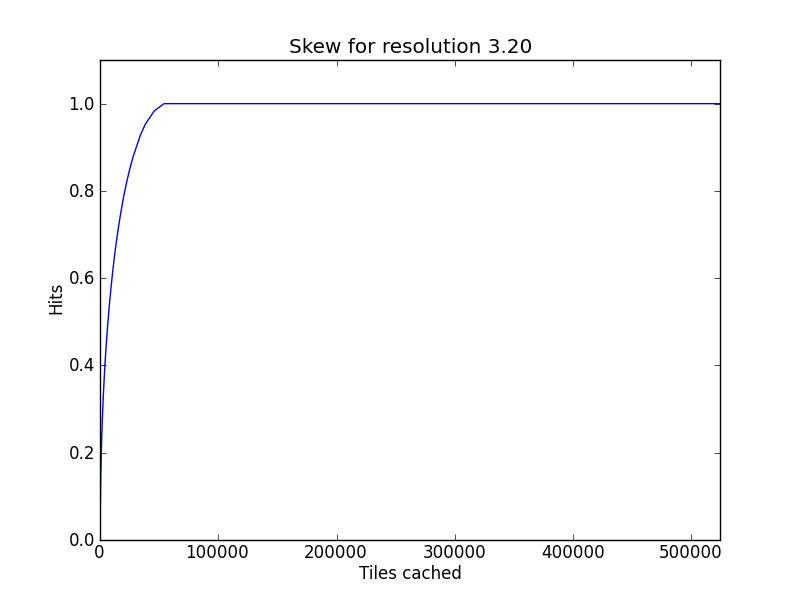
\includegraphics[scale=0.5]{skew-3_2.png} & 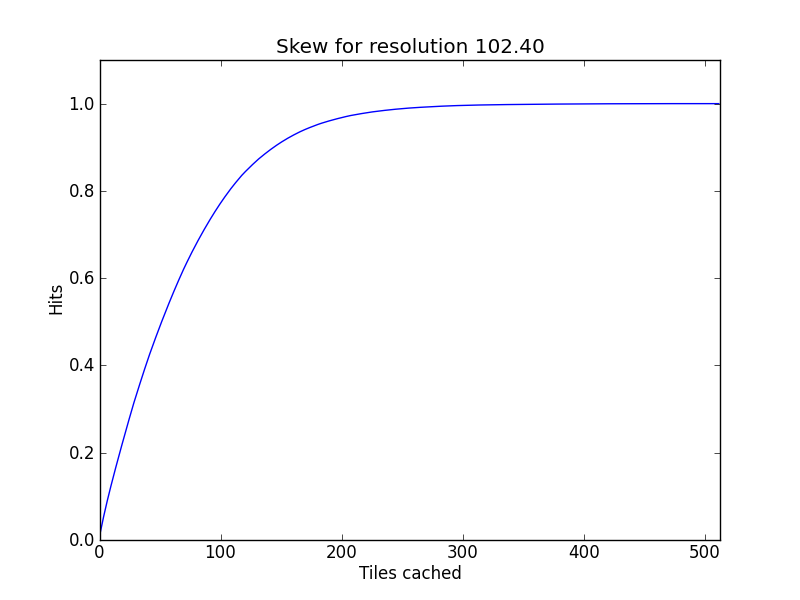
\includegraphics[scale=0.5]{skew-102_4.png} \\
%\end{tabular}
%\caption{Cummulative function of tile access frequency for high resolution (top) and low resolution (bottom) tiles. The skew is stronger for the high resolution.}
%\label{fig:skew}
%\end{figure*}
